%%Maximum length = smallestOf( 12,000 words, 35 pages )
%%Report file name must be "team_X.pdf" (where X is the team name)

%Your initial report set out your aims for the project which you may wish to modify in light of feedback received. The final report should detail out what you set to achieve, what you did achieve, how you achieved it, and your evaluation of your work. You are free to structure your report as you see fit, and different projects may naturally lead to different structures. An example structure for your report follows. Bear in mind that the main aim of your report is to show the examiners that you have done quality work: focus on the noteworthy, not the mundane; explain what the examiners cannot know rather than the obvious; and show that you understand your project’s weaknesses as well as its strengths.


% Apply paragraph spacing only for the main report body %
\setlength{\parskip}{1em}

\section{Introduction}
%Describe the context for the work and the problem you are addressing. Briefly summarise what you achieved in the project.

\begin{itemize}
	\item Context
	\begin{itemize}
		\item Road traffic simulator
		\item Goal was to simulate road traffic on urban networks to enable some general data gathering and be able to plugin more specific metric recorder for pollutants, throughput load on junction, etc...
		\item ES::NOTE: maybe do a comparison with the goals set out in the original report?
		\item Originally started as a cell automata micro model
		\item Model became too restrictive as cells were of fixed lengths and model was not easily scalable
		\item Morphed to encompass features of macro model and agency principles
	\end{itemize}
	\item summary of chevos
	\begin{itemize}
		\item Hybrid model
		\item map objects as agent that decide their behaviours based on environment
		\item focus of design was about solid foundations so that the software can be expanded upon without any major structural changes
		\item i.e.: very expandable without needing to change the core design
		\item Maps imported from real-life OpenStreetMap (OSM) data so realistic
		\item Maps can also be created synthetically as long as the format is the same
		\item allows for real world usage off-the-shelf
		\item PIC of the app!!!
	\end{itemize}
\end{itemize}

\section{Review}
%Describe related work.

Many different software traffic modeling systems were developed.
Some of them are using classical software modeling approaches, some of them are based on innovative and hybrid approaches.
Both have advantages and disadvantages.
In this chapter we will briefly highlight strong and weak sides of those software implementations
and a theory which are they based on.

\begin{itemize}
    \item SUMO -  microscopic approach
    \item MATsim - microscopic agent-based approach
    \item AIMSUN - hybrid approach
    \item SIDRA - macroscopic approach
\end{itemize}

Simulation of Urban MObility (SUMO) is a popular open-source road traffic simulation software which was implemented using the aspects of microscopic flow behavior model.
The main idea is to simulate complex road networks. Any road network can be represented by importing or creating various sources [academia].
Being a classical microscopic based simulator SUMO supports a simulation of such parts of traffic as ways, junctions, traffic lights, routes.
Also appropriate demands can be created. Like physical properties of vehicle, logical parameters and vehicle type distribution.
There are many different options supported by SUMO.
SUMO is open and well studied software. Also it was implemented in different national projects[main site].

Sumo minus

Despite being widely used SUMO one of the most significant disadvantages of SUMO is its complexity.
This requires users to spend more time in order accurately set
all parameters and understand aspects of micro-simulation more comprehensively. [academia]




AIMSUN is another popular and well studied, but commercial
transport simulation software made by Transport Simulation Systems in Spain.[main site]
It is commonly classified as a microscopic based simulator.
Nevertheless it also supports simulation of macro and meso models.
Depending on which model the user is intended to simulate he/she can configure specific mode and manage the traffic flow[nz].
Supporting a dynamic simulation AIMSUN can operate with larger road networks as highways, freeways, and ring roads.
By default it has simulation scenarios which allows user to run experiments with specific parameters.

Anohter feature  supported by AIMSUN is 3d simulation which provides detailed point of observation from any angle.

AIMSUN minus

On of the significant disadvantages of AIMSUN is the longer coding phases which
requires users to spend more time for coding rather than set the settings.
Also as it was said [] usage of 3d modes dramatically affects the performance.[masse.ac.nz]

 MATsim -
 SIDRA -


\section{Requirements and Design}
\begin{itemize}
    \item Flexible requirements - start with something basic, get to more complex (stage 2 possibilities.)
    \item Model evolved from simple cellular-automata with discrete cells occupied by cars (or free) to more physics-like model, with the cars having position and bearing in real world map, moving along the lanes, with position and sizes resembling real like and set as floating-point numbers
    \item Started with one set of requirements - traffic lights, self-driving cars - but ended up with 1. real life map model (roads, lanes, crossings) 2. simpler car behaviour (no traffic lights, random decision as to go forward on crossing or turn) 3. much more comprehensive GUI (map pane with zoom/pan, on-map selection with mouse, different rendering settings such as debug roads, debug crossings, etc.) 4. more complex vehicle movement model - acceleration/deceleration, distance to keep.
	\item ES::NOTE: maybe original pic of the 3 modules here?
	\item >> Separation of concern principles
	\item >> focus on solid bases to enable expandability and real world usage?
\end{itemize}

%Describe the requirements you set for your project at the beginning and the design you have taken for your project. Focus on why you decided to tackle the problem in the way you did, and what effects that had on the design. You may also wish to mention the impact of team-working on your requirements and design.


\section{Implementation}
%Describe the most significant implementation details, focussing on those where unusual or detailed solutions were required. Quote code fragments where necessary, but remember that the full source code will be included as an appendix. Explain how you tested your software (e.g. unit testing) and the extent to which you tested it. If relevant to your project, explain performance issues and how you tackled them.

%%%%%%%%%%%%%%%%%%%%%%%%%%
% Alex part
%%%%%%%%%%%%%%%%%%%%%%%%%%
%%%%%%%%%%%%%%%%%%%%%%%%%%
\subsection{Technology and libraries}
\begin{itemize}
    \item Java SE 1.8
    \item most of the actual simulation and drawing code is written manually
    \item libraries used: main code: Java standard library \(rt.jar\), testing code: jUnit, Mockito, Fest-assert. Own logger used.
    \item OSM for the import map data
\end{itemize}

%%%%%%%%%%%%%%%%%%%%%%%%%%
% Alex part
%%%%%%%%%%%%%%%%%%%%%%%%%%
%%%%%%%%%%%%%%%%%%%%%%%%%%
\subsection{Map data import (OSM)}
According to the requirements, the software would need to be able to model traffic behaviour in real-like road networks. In addition to the organic requirements needs, there were synthetic type of requirements demanding for various test fixtures for all application components from actual vehicle behaviour to individual lane visualisation.

Decision was made to use already-available public-domain ordnance data from OpenStreetMap\footnote{OSM data is available under ODbL license, see http://www.openstreetmap.org/copyright} (OSM)  worldwide project. It was a natural decision since data is available for all the world, and is collaboratively created by multitude of users, OSM has a strong technical community and ample documentation, and, finally, it contains all the data which may be required for traffic simulation. In addition to that, data files are available in well-known XML format\footnote{Having said that, there is no official XML type specification due to main software pieces in ecosystem vaguely interpreting different cases: http://wiki.openstreetmap.org/wiki/OSM\_XML}. As an extremely useful side-effect, using such widely available data allows a user to obtain a map of the area of particular interest for simulation following simple steps, so it greatly adds to the practical value. At the same time, the implementation of such loading turned out to be not straightforward due to data originating from many human contributors bearing all the inconsistencies and errors possible for vaguely defined data.

OSM format defines three main types of objects: nodes (points having coordinates), ways (polylines, sequences of nodes) and relations (types of relationships between other objects), which are extensively tagged, to represent all the complex setting of the real-world mapping. For example, a way (sequence of node references) with tag type equal to primary and lanes equal to 4, would mean a two-way primary road. A way with type building represents a building on the map, and should be a closed polygon. All the objects have the ID attached to them.

Following is a compact overview of the pipeline data follows from the OpenStreetMap file downloadable from the internet to the actual simulation process:
\begin{itemize}
    \item Stage 1. Using standard OSM software tools (Osmosis, JOSM), prepare the excerpt from large data set suitable, which is suitable for simulation.

    \item Stage 2. Using obtained OSM XML file, load a set of Descriptor objects:
    \begin{itemize}
        \item Collection of road descriptors: objects describing roads, with number of lanes in each direction
        \item Collection of junction descriptors: object describing junctions, and their connection with roads
        \item Generic knowledge about map setting, such as map geographical bounding box.
    \end{itemize}

    \item Stage 3. Using descriptor objects, construct in-memory graph representation of the road networks:
    \begin{itemize}
        \item Create roads from descriptions. Create individual lanes within the roads. Offset lanes accordingly.
        \item Create junctions from descriptors.
        \item Link roads and junctions using junction descriptors. Link on individual lanes. Compute possible inflow and outflow paths for junctions to save time in simulation run.
        \item Walk the graph and attach traffic generators and receivers to not yet connected edges.
    \end{itemize}

    \item Stage 4. Run the traffic simulation on the created map.
\end{itemize}

%%%%%%%%%%%%%%%%%%%%%%%%%%
% Alex part
%%%%%%%%%%%%%%%%%%%%%%%%%%
%%%%%%%%%%%%%%%%%%%%%%%%%%
\subsubsection{Preparing data file}
First of all, user needs to decide on the actual geographical area they want to perform simulation in. The area is uniquely defined by 2 pairs geogrphical of coordinates in latitude, longitude coordinate system: (south-west lat, long) - (north-east lat,long). After that, user needs to either download the full planet.osm file (containing whole OSM data set), or an area excerpt containing area of interest\footnote{Geofabrik is a reliable source for OSM excerpts with fresh data http://www.geofabrik.de}.

Following is the osmosis tool command line, which combines both cut and filter steps into single run:
\begin{lstlisting}
$ osmosis --read-xml file=INPUT_LARGE_FILE.osm enableDateParsing=no
        --tf accept-ways highway=trunk,motorway,primary,secondary,tertiary
            ,motorway_link,trunk_link,primary_link,secondary_link,tertiary_link
        --bounding-box bottom=48.867844 left=2.289727 top=48.879678 right=2.304442 completeWays=yes
        --used-node
        --write-xml OUTPUT_FILE.osm
\end{lstlisting}
'completeWays=yes' key is of specific interest. When osmosis attempts bounding box reduction, and finds a way which is located both inside and outside the bounding box, its default behaviour is to terminate the way at the last node within the box. When applied to real life data, this yielded ugly results, sometimes terminating road network segment where it should not terminate. As a counter action, this key is used to include all the ways which are within, or intersect with, bounding box rectangle.  As a result, we obtain an OSM XML file with some ways spanning outside of the box, which may be opened directly from within the user interface of the Traffic Simulator system, or edited in any standard OSM file editor, such as JOSM.

Figure \ref{fig:thirdPartyToolsOSMPreparation} summarizes steps performed during prelminary file preparation process.
\begin{figure}[h]
    \caption{Process of preparing the OSM xml file using OSM tools}
    \label{fig:thirdPartyToolsOSMPreparation}
    \centering
    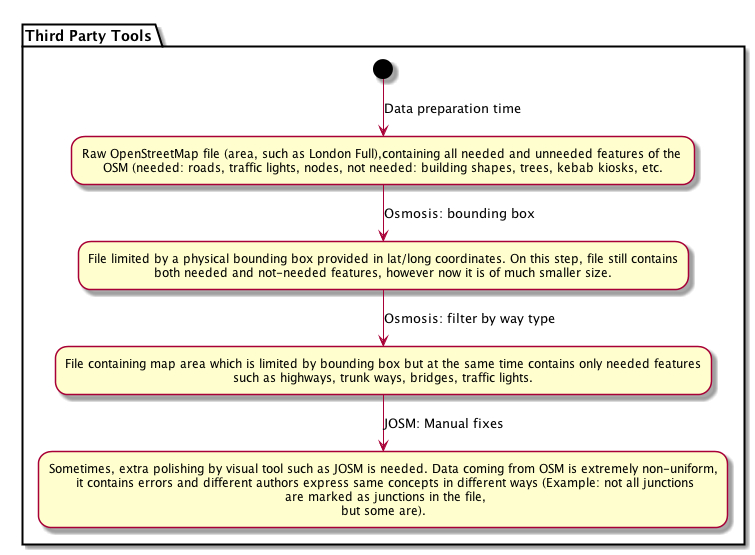
\includegraphics[width=0.8\textwidth]{../../uml_diagrams/thirdPartyToolsDataLoading.png}
\end{figure}


%%%%%%%%%%%%%%%%%%%%%%%%%%
% Alex part
%%%%%%%%%%%%%%%%%%%%%%%%%%
%%%%%%%%%%%%%%%%%%%%%%%%%%
\subsubsection{Descriptors creation from the OSM file}
After the actual simulation map OSM file is created, it may be opened directly from traffic simulation. In order for the data contained in an XML file to be used, it first needs to be read, parsed and adopted into the internal format, and also linked into the in-memory graph.

Actual parsing of the XML file has been implemented using standard java SAX\footnote{Simple API for XML, https://docs.oracle.com/javase/7/docs/api/javax/xml/parsers/SAXParser.html} parser. When choosing between the DOM and SAX parsing, the latter was selected with no doubt, since the DOM has significantly larger memory requirement as soon as it establishes the whole document as tree in memory, and exposes many complex APIs and methods for manipulation which are not needed for the loading data case. SAX employs event-driven XML parsing model: when parser encounters new element, closing element, an attribute or text blocks, it invokes appropriate methods on handler object. In order to listen to these events, class OsmSaxHandler has been created.

From the XML file, first the bounding box is read, the actual geographical rectangle containing all the places of interest. Whilst OSM operates in geo-coordinates, actual simulation happens on a flat Cartesian coordinate system first quadrant map. All objects have coordinates as offset from zero point by x and by y axis. Figure \ref{fig:coordinateConversions} provides an overview of what are the coordinate systems used across the traffic simulation system. On this stage of parsing, conversion operator is initialized for geographical to meters offset coordinate system conversion.

\begin{figure}[h]
    \caption{Coordinate systems used in traffic simulation system}
    \label{fig:coordinateConversions}
    \centering
    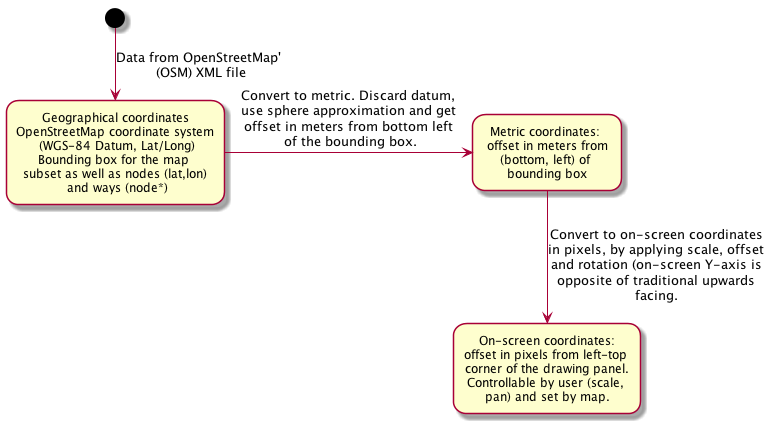
\includegraphics[width=0.8\textwidth]{../../uml_diagrams/coordinateSystems.png}
\end{figure}

 Since OSM has quite few basic objects to express mapping data, roads are expressed as <way> elements, containing sequence of references to nodes, effectively forming a polyline. There is no notion of road width in original data, only the number of lanes and if the road is one way. The design decision has been made to default lane width to standard 3.2 meters. Using lane width, one-way flag and number of lanes in road, physical representation of road is created.

\begin{figure}[h]
    \caption{Polyline creation and visualisation stages}
    \label{fig:roadAndLanesPolylines}
    \centering
    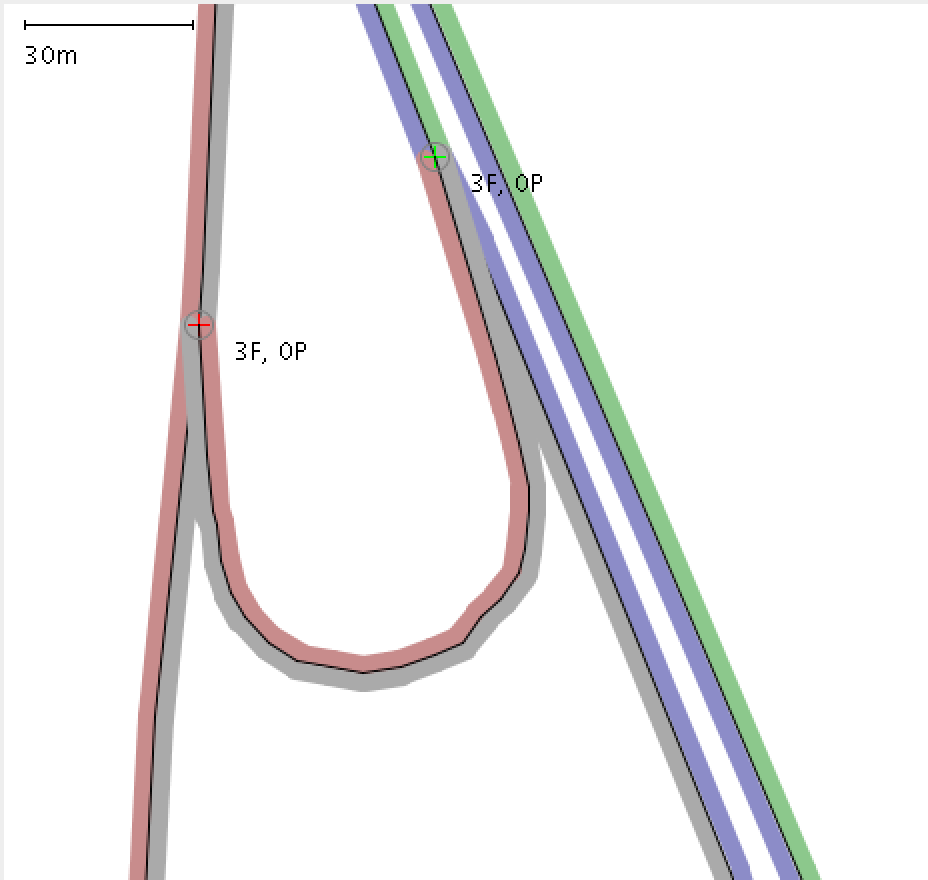
\includegraphics[width=0.4\textwidth]{figs/road/road_polyline.png}
    \hspace{0.2em}
    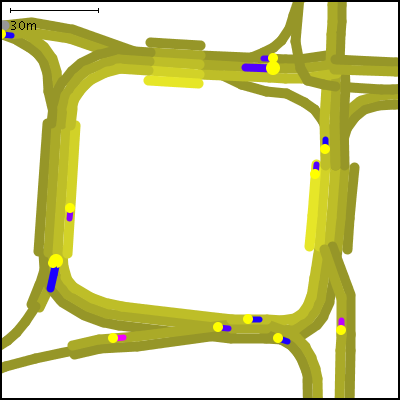
\includegraphics[width=0.4\textwidth]{figs/road/road_lanes.png}
\end{figure}

At the same time, XML data file provides enough information to construct a central road axis polyline. After this polyline is available, polylines for the individual lanes are constructed, using positive or negative shifts along thr normal vector to current segment of the polyline, with the shift amount depending on the position of the lane in road. Figure \ref{fig:roadAndLanesPolylines} provides an overview of the process: on the left the road central axis polyline is visible (thin black hairline), on the right the more complex junction with multiple lanes, constructed using the method mentioned before.

For the simulation to run smoothly, the road networks needs to be represented as a well-formed graph data structure. In order to facilitate the requirement, post-processing is applied to the road and junction descriptions collected from the XML file. Roads containing junction node as a non-edge polyline node were split - one part terminating at junction whilst the other starting from it. This allowed for future uniformity of the movement logic. The vehicle simply follows high-level graph while making low-level decision on acceleration and deceleration and is naturally transported to the next feature (graph node) as long as it terminates previous one.

Unfortunately, the collaborative nature of OpenStreetMap data leads to multiple ambiguities:
\begin{itemize}
    \item Human factor. Same real-world concepts, such as junctions, road connections and pedestrian crossing, happen to be expressed in a different way in XML file by different contributors. For example, the node has a tag which indicates that it is a junction, however not all real crossings do have this label attached to the crossing node. The design decision has been made to default to the least common denominator, and simply consider a situation when same node identified by the id is contained in two ways a crossing.
    \item Eventual data consistency. In some cases the OpenStreetMap data contains simple errors or misconceptions, which led to the concrete changes in coding practice: for example, instead of throwing an exception when meeting an inconsistent data situtation, the load layer attempts to fix it to best possible degree available to it, extensively logging the causes and related data excerpts for human inspection. For example, if the node referenced in the road polyling is not found in data file, the data loading is not terminated - some nodes just happen to be cut off by processing, and some are erroneously referenced. It seems that official OSM software is tolerant to these inconsistencies as well, and presence of such ill-formed data is one of the causes of the absence of the formal data specification.
\end{itemize}

The approach of importing OpenStreetMap data was eventually found to have some similarities to the one employed in SUMO system, with some use of guess work as well as high tolerance to the data file errors. At the same time, SUMO employs much more complex and rich data standard for its simulation setting.

Following problems were encountered and solved during the implementation of the XML data loading:
\begin{itemize}
    \item Coordinate conversions. Since the Mercator projection with spherical geoid simplification is used, there is certain inaccuracy in coordinates converted to meters offset.
    \item Splitting roads having junctions in the middle of the road. Rather a technical complexity, it led to a cumbersome algorithm, since the processing of the roads and junctions happened at the same time, so in case of the split it is required to ensure that all references to split road are updated to either part of it.
    \item Link descriptions. Initially, it was anticipated that another type of descriptors - Link descriptors - would be created to mark the places where two parts of the road are connected (for example, pedestrian crossing on a straight road). However, after the implementation of the data loading found out a need for road splitting, Link descriptors had to be abandoned in favour of more general idea of junction descriptors having only two roads connected. Otherwise, the edge-case situation of a link descriptor created in a geographical point, which was later to be found to be in the middle of another road led to an overly complex code handling this edge cases. This conversion only positively reflected on the overall design of the system, following "keep it simple" rule. Later stage of the graph construction and actual simulation were found working perectly with junctions of two roads acting as links.
    \item Lane construction. Deriving from a single zero-width road polyline a set of lane polylines which are offset into appropriate direction (perpendicular to the segment).
\end{itemize}

At the same time, extending the map data loader with extra functionality, such as maintaining pedestrian crossing information or traffic lights information, would provide system with some benefits, there is a clear potential for improvement on this side.

\subsection{Graph construction}

Graph construction is done prior to the simulation running rather than during (JIT). This approach moves the performance penalty away from the live simulation leaving some overhead for large workload heavy maps. it also, conceptually, makes for easier storage of map states on every tick as, once the graph is set, the only changes are in the counters, link states (e.g.: such as traffic lights being red/green) and the map objects travelling on the graph.
From the previously created descriptors, the graph constructor creates the features and links of the graph and links them together in this order (see Figure~\ref{fig:graphConstructSeqDiag} and ~\ref{fig:roadConstructSeqDiag} in Appendix~\ref{sec:roadConstructionSequences}):
\begin{enumerate}
	\item Roads, their directed lane groups and individual lanes are created,
	\item Junctions are created and the roads branching off them connected,
	\item Traffic generators are placed.
\end{enumerate}

\subsubsection{Feature creation and linkage}

Originally the graph was kept abstract with features connected via links (see Figure~\ref{fig:FeatureConnect}). These features could be either junctions or roads. Roads were connected as whole features (see Figure~\ref{fig:RoadsOriginal}).

\begin{figure}[h]
	\vspace{1.5em}
    \caption{Original design with Features and Links}
    \label{fig:FeatureConnect}
    \centering
    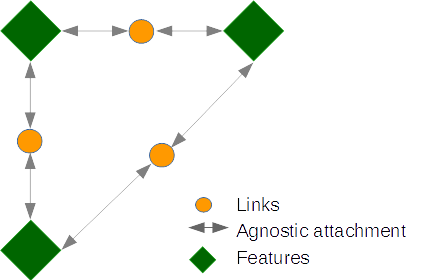
\includegraphics[width=0.50\textwidth]{figs/graphConstruction/OriginalConnections.png}
    \vspace{1.5em}
\end{figure}

\begin{figure}[h]
    \vspace{1.5em}
    \caption{Roads in the original high abstraction design}
    \label{fig:RoadsOriginal}
    \centering
    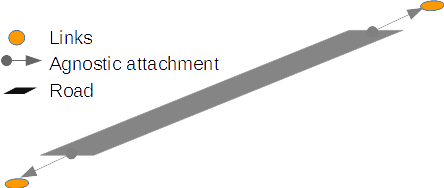
\includegraphics[width=0.45\textwidth]{figs/graphConstruction/OriginalRoads.png}
    \vspace{1.5em}
\end{figure}

As more work was done it became clear that this high level of abstraction on the graph was not going to be practical. Thus it progressed into having roads broken into groups of directed lanes. This allows the lanes to be connected individually in a directed fashion in the graph. Roads are now composed of lane groups that are, themselves, composed of single lanes (see Figure~\ref{fig:RoadsFinal}).

\begin{figure}[h]
	\vspace{1.5em}
  	\caption{Roads, Directed lane group and lanes}
  	\label{fig:RoadsFinal}
  	\centering
	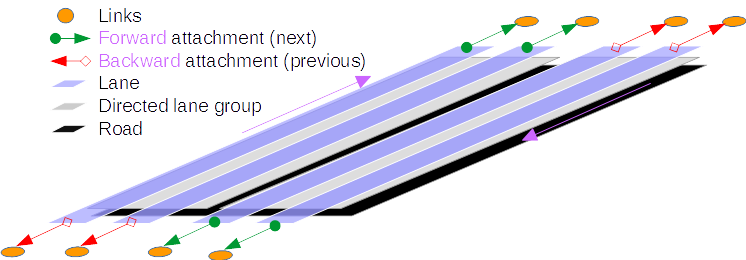
\includegraphics[width=0.75\textwidth]{figs/graphConstruction/Roads.png}
  	\vspace{1.5em}
\end{figure}	

Although roads and lane groups are not directly connected up in the graph, the belonging lanes can back reference those enabling travelling objects to access their properties. I.e.: A vehicle on a lane can find out the Road's name or ID as well as what direction it belongs to.

Junctions were developed around this exploded view of the road feature. Lanes are connected up to junctions via special junction specific links that give access to available paths from that particular entry point with the <getLinks()> method for any passing objects (see Figure~\ref{fig:junction}).

\begin{lstlisting}[language=Java]
    public List<Link> getLinks() {
        try {
            return junction.getNextLinks(super.getID());
        } catch (JunctionPathException e) {
            LOG.log_Fatal("No exit link from the junction were found! i.e.: Car is stuck!");
            return new ArrayList<>();
        }
    }
\end{lstlisting}

Paths are calculated after lane linkage has been done. All entry points are connected up to all exit points unless it double backs on the same road (u-turn) (see Figure~\ref{fig:junction}). The paths are stored in a <TrafficBehaviour> object as lists for each entry point ID inside a map:

\begin{lstlisting}[language=Java]
	private Map<ID, List<ID>> outflowPaths;
\end{lstlisting}

\begin{figure}[!h]
	\vspace{1.5em}
  	\caption{Junction}
  	\label{fig:junction}
  	\centering
	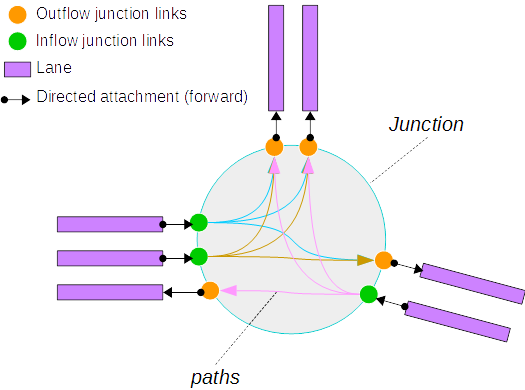
\includegraphics[width=0.6\textwidth]{figs/graphConstruction/Junction.png}
  	\vspace{1.5em}
\end{figure}

\begin{itemize}
	\item link descriptions are depreciated after work on the OSM showed that universal linkage with junctions were for easier to do then identifying what was 1-to-1 link or a junction from the OSM data
\end{itemize}

\subsubsection{Traffic Generators}

Traffic generators were originally designed to only produce traffic but evolved to also take receipt of it thus taking on the responsibility of deleting vehicles as they exited the boundaries of the simulated map. This ensures that vehicles cannot keep going (graphically) and disappears at the designated boundaries. This also allows to keep track on the numbers of vehicles produced and received at those points (see Figure~\ref{fig:boundaryTF}).

During development two corner cases were encountered:
\begin{enumerate}
	\item Junctions were there were only incoming lanes connected to,
	\item Junctions were there were only incoming lanes connected to save for one road.
\end{enumerate}

In the first case, vehicles from all lanes had no where to go. In the second case, where the traffic came into the junction from the lone road with both direction included, the traffic had also no where to go since the only way out would have been a u-turn which is not allowed.
Both were dealt by placing traffic generators on those special case junctions to take in the orphaned traffic (see Figure~\ref{fig:junctionTF}).

\begin{figure}[!h]
	\vspace{1.5em}
	\centering
	\begin{minipage}[t]{0.60\textwidth}
  		\caption{Traffic Generators at Map boundaries}
  		\label{fig:boundaryTF}
  		\centering
		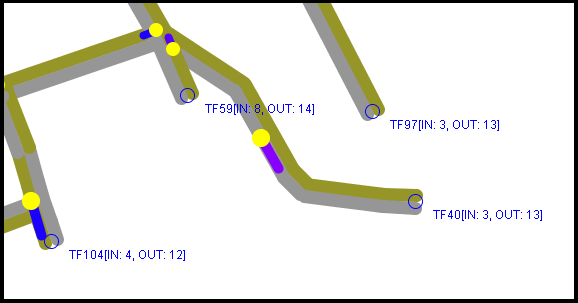
\includegraphics[width=1\textwidth]{figs/trafficGenerator/generate-receive.png}
	\end{minipage}\hfill
	\begin{minipage}[t]{0.35\textwidth}
  		\caption{Junction Traffic Generator}
  		\label{fig:junctionTF}
  		\centering
		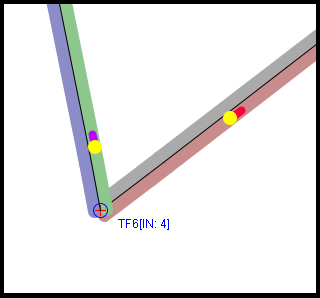
\includegraphics[width=1\textwidth]{figs/trafficGenerator/inflowOnly.png}
	\end{minipage}
	\vspace{1.5em}
\end{figure}

By having traffic generators automatically placed at any dangling links, any OSM data issues or inconsistencies can be seen in the graphical representation of the map at a glance. It also acts as a safety net when these occur by ensuring that all ends are connected to something and traffic is kept within the boundaries of the map (i.e.: no escaping vehicles). Another positive side effect is that, during construction of the graph, any island features (be it orphaned features that are unconnected or actual geographic islands) are ensured to have traffic running on them. For example see Figure~\ref{fig:islandReal}.

\begin{figure}[!h]
	\vspace{1.5em}
  	\caption{Island problem resolution}
  	\label{fig:islandReal}
  	\centering
	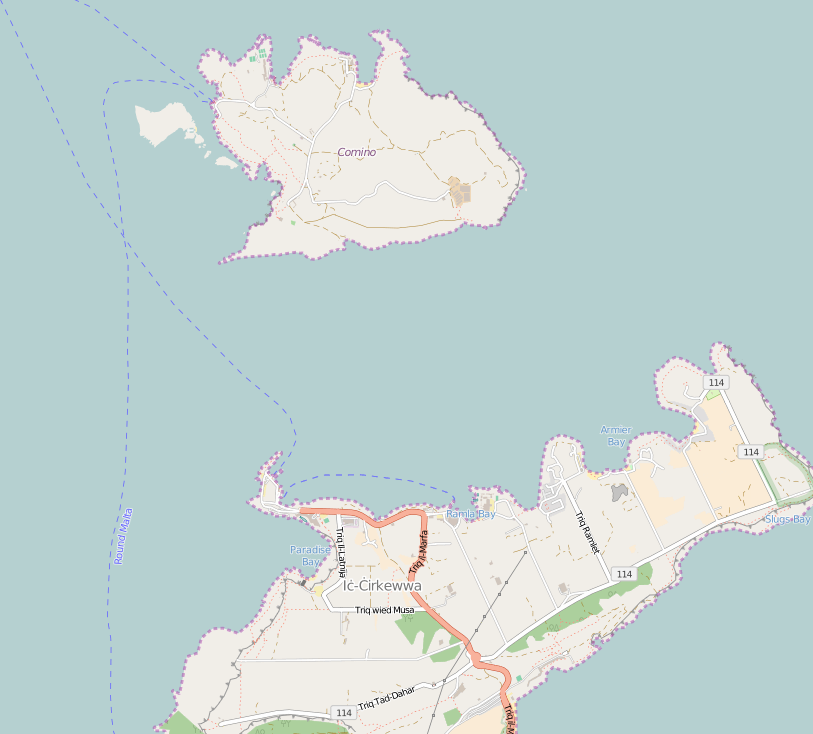
\includegraphics[width=0.4\textwidth]{figs/trafficGenerator/IslandExample_realmap.png}
	\hspace{0.2em}
	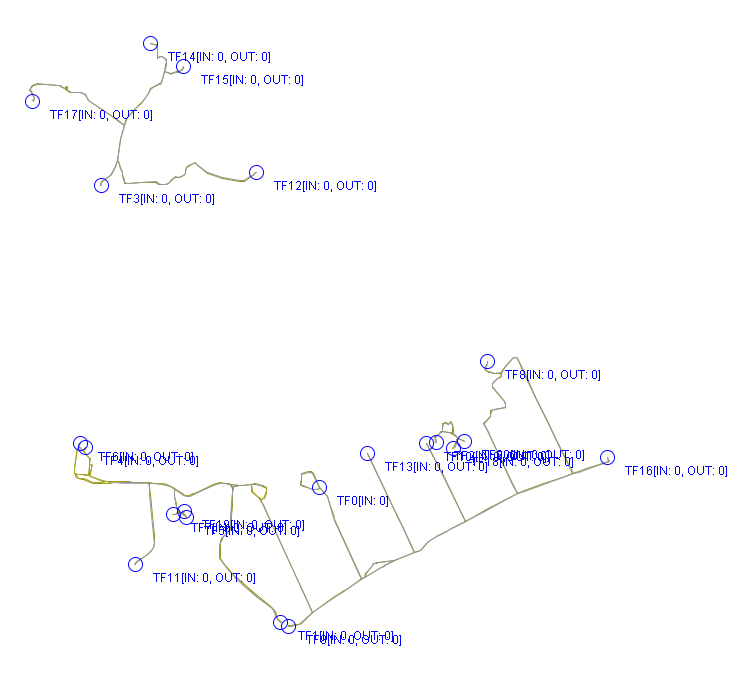
\includegraphics[width=0.40\textwidth]{figs/trafficGenerator/IslandExample_simmap.png}
  	\vspace{1.5em}
\end{figure}

\subsubsection{Traffic Lights}
\begin{itemize}
    \item two types of traffic lights: singles and those in one junction set
    \item all traffic lights work autonomously
	\item traffic light state: discussion whether traffic light State should be boolean or enum \(everyone wrote his version of boolean traffic lights, different ideas so we have taken Enum\)
\end{itemize}

\begin{itemize}
        \item traffic lights rules are basic, they do not change states according to the traffic (not intelligent traffic lights)
        \item only two states in traffic lights: red and green, we do not have early/late yellow etc.
\end{itemize}
     
\begin{itemize}
	\item serialization/de-serialization
\end{itemize}

\subsubsection{Caveats}
\begin{itemize}
	\item Problems:
	\item > issues streaming from the OSM data leads to bug where in a round about a incoming road cannot be connected up
	\item > Example!! + PIC + explanation as to why exactly
\end{itemize}


%%%%%%%%%%%%%%%%%%%%%%%%%%
% Alex part
%%%%%%%%%%%%%%%%%%%%%%%%%%
%%%%%%%%%%%%%%%%%%%%%%%%%%
\subsection{Map visualisation}
\begin{itemize}
    \item Map visualisation
    \begin{itemize}
        \item Coordinate conversion - meters-offset to pixels x/y (on-screen). This is the view-centric coordinate system which depends on scale, movement, size of window.
        \item Vehicle specific coordinates: lane it belongs to AND position along the polyline.
        \item GUI features: map zoom, pan, scale.
            \begin{figure}[!h]
                \vspace{1.5em}
                \caption{Map zoom options}
                \label{fig:mapZoomOptions}
                \centering
                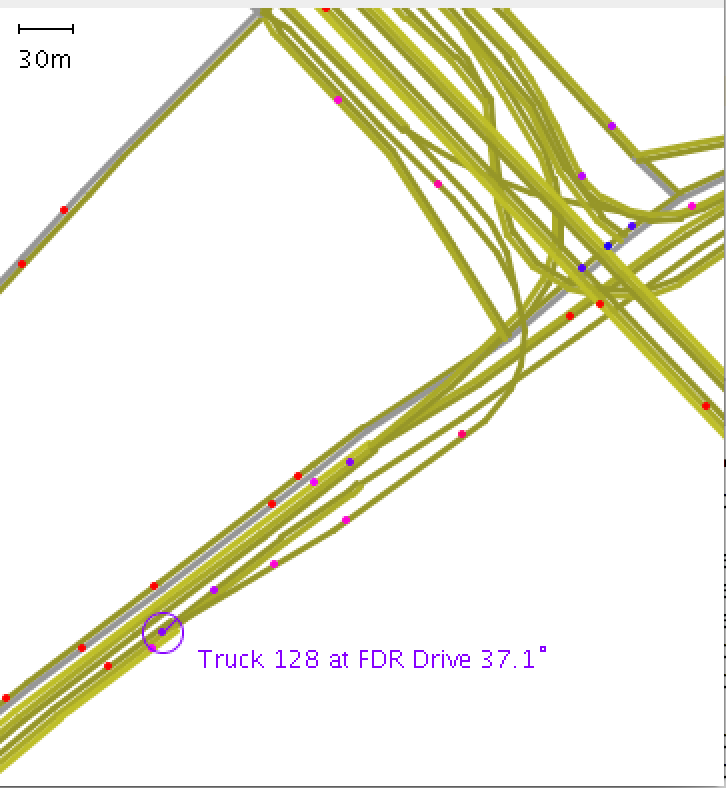
\includegraphics[width=0.4\textwidth]{figs/road/zoom_dots.png}
                \hspace{0.2em}
                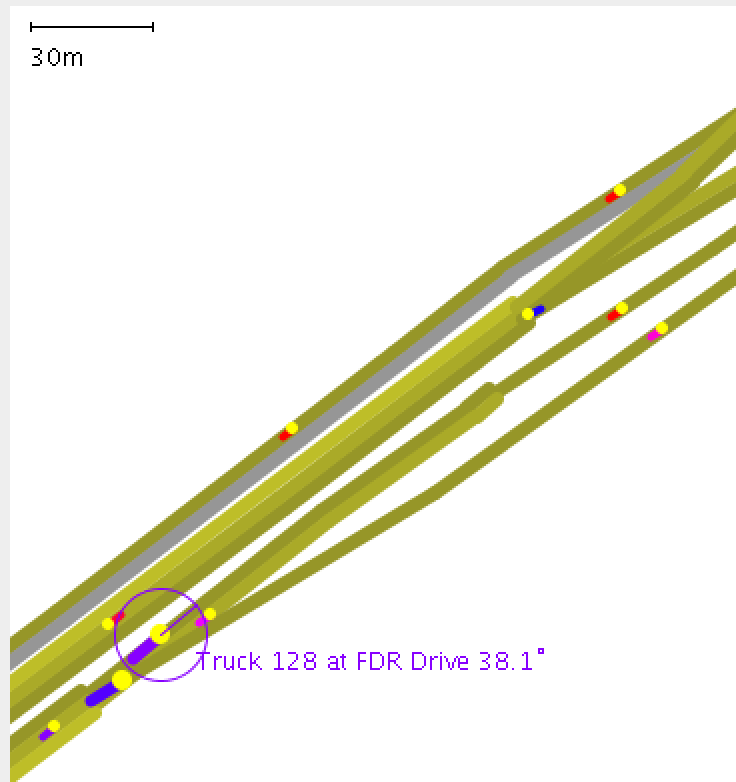
\includegraphics[width=0.4\textwidth]{figs/road/zoom_cars.png}
            \end{figure}

    \end{itemize}
\end{itemize}


%%%%%%%%%%%%%%%%%%%%%%%%%%
% Alex part
%%%%%%%%%%%%%%%%%%%%%%%%%%
%%%%%%%%%%%%%%%%%%%%%%%%%%
\subsection{Vehicle movement}
\begin{itemize}
    \item How vehicle moves: physical model (speed, acceleration, direction, distance.)
    \item Speed limits, two types of cars
    \item Car belongs to a lane. How coordinate conversion happens (poing, angles, distnace.)
    \item Moving on a lane, changing lanes:
        \begin{figure}[!h]
            \caption{Car changing lane}
            \label{fig:carKeepingDistance}
            \centering
            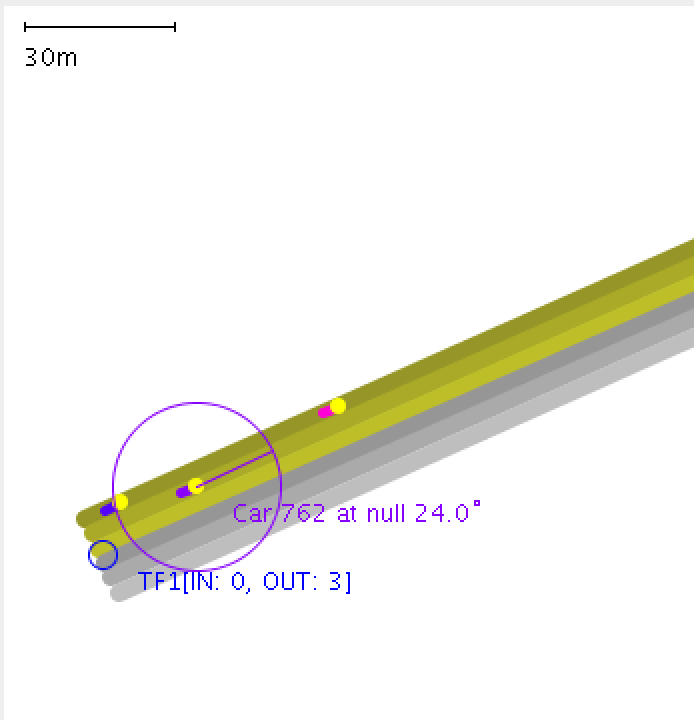
\includegraphics[width=0.3\textwidth]{figs/carMovement/car_keeping_distance_to_other.png}
            \hspace{0.2em}
            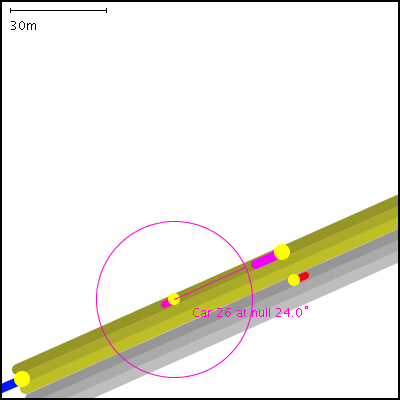
\includegraphics[width=0.3\textwidth]{figs/carMovement/car_lane_change_before.png}
            \hspace{0.2em}
            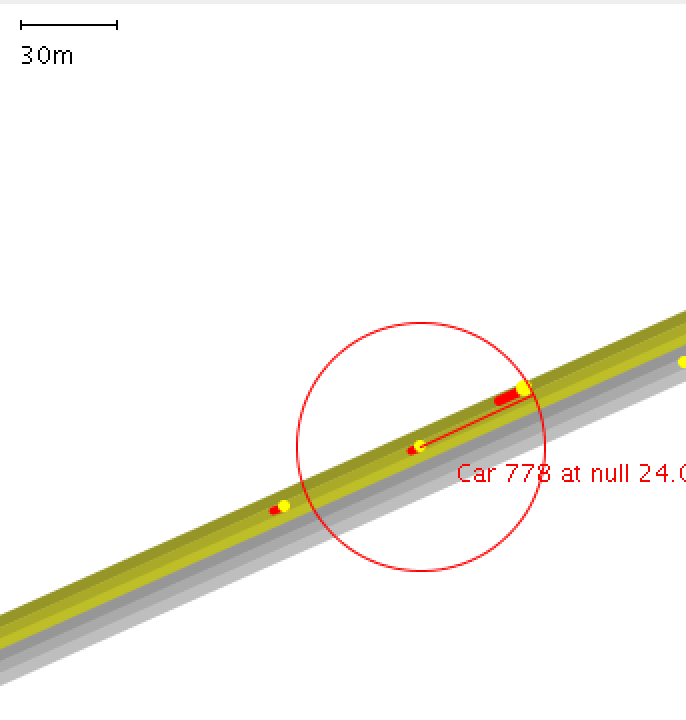
\includegraphics[width=0.3\textwidth]{figs/carMovement/car_lane_change_after.png}
        \end{figure}

    \item What vehicle should do when reaching junctions
    \item Junctions and possible outcomes for vehicle
        \begin{figure}[!h]
            \caption{Junctions found in real life}
            \label{fig:junctionTypes}
            \centering
            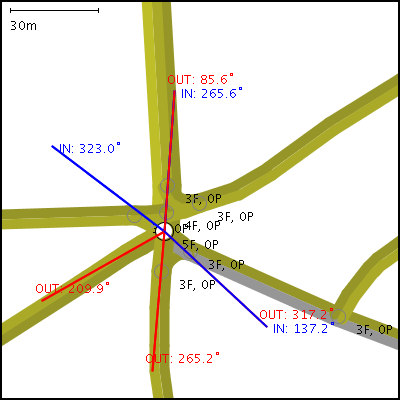
\includegraphics[width=0.4\textwidth]{figs/junction/junction_5_roads.png}
            \hspace{0.2em}
            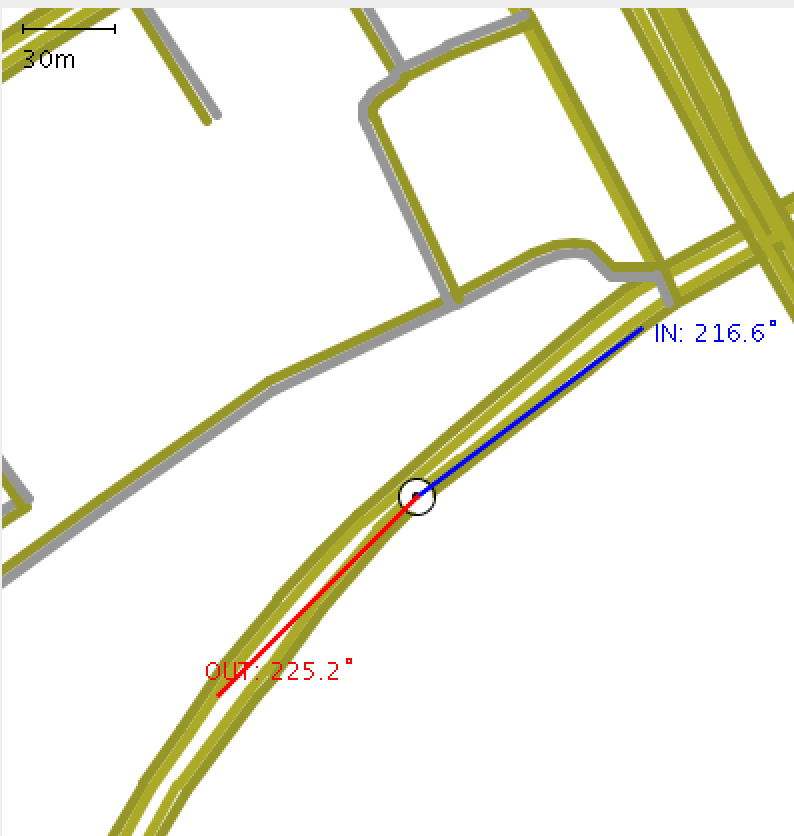
\includegraphics[width=0.4\textwidth]{figs/junction/junction_two_roads.png}
        \end{figure}

        \begin{figure}[!h]
            \caption{Types of forks found in real life }
            \label{fig:forkTypes}
            \centering
            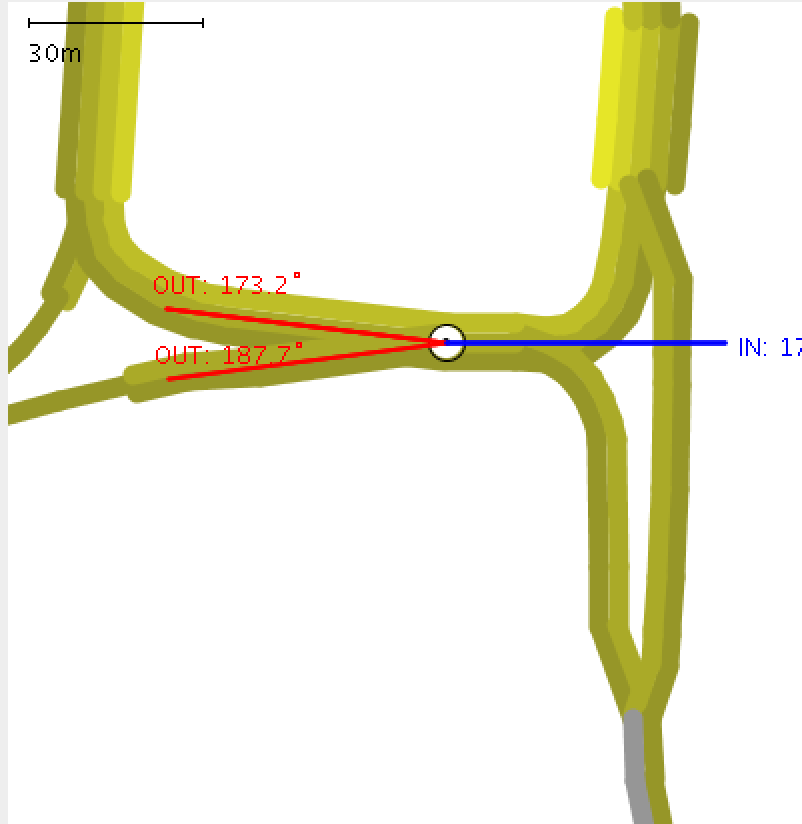
\includegraphics[width=0.4\textwidth]{figs/junction/junction_oneway_to_fork.png}
            \hspace{0.2em}
            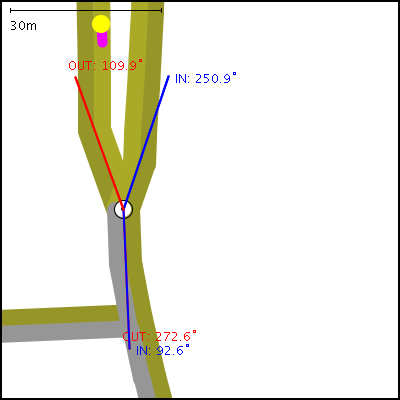
\includegraphics[width=0.4\textwidth]{figs/junction/junction_two_way_to_fork.png}
        \end{figure}

    \begin {itemize}
        \item our model: junctions 1-type: only 2 roads connected
        \item our model: junction 2-type: more than 2 roads connected (actual junctions)
            \begin{figure}[h]
                \caption{Junction forward or turn options depending on angle }
                \label{fig:forwardOrTurnOption}
                \centering
                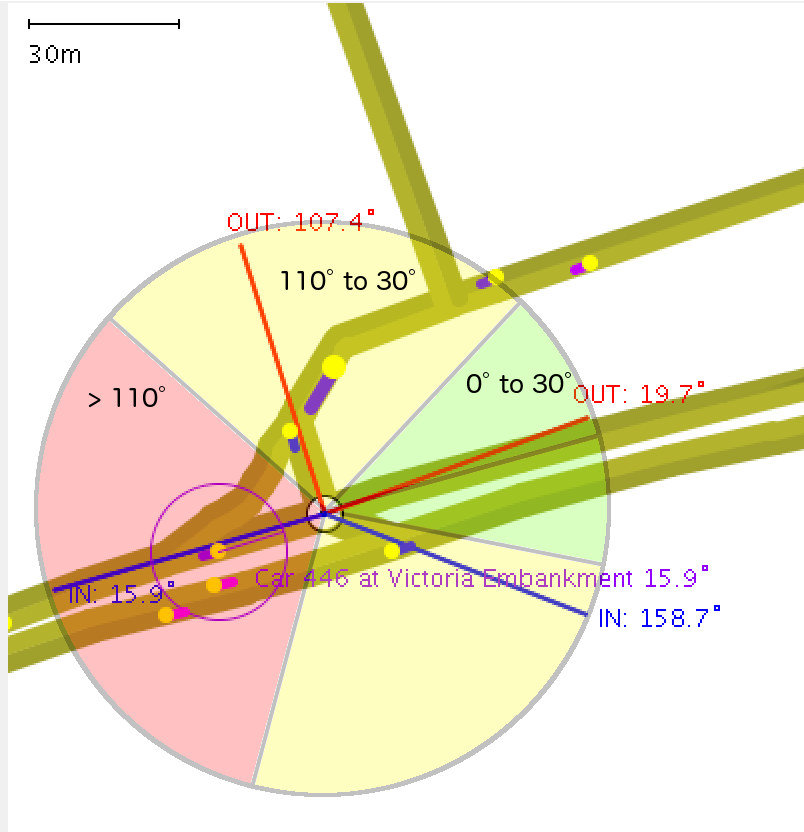
\includegraphics[width=0.4\textwidth]{figs/junction/junction_car_incoming_angle_with_turn_sectors.png}
            \end{figure}
        \item explain incoming lane angle, outgoing angles and its effect on vehicle movement - what is considered straight movement, and what is considered turn. >110 is prohibited, 110-30 is turn 30-0 is straight. This enforces us to skip weird turns at forks, for example.
    \end {itemize}
\end{itemize}


\subsection{Logger}

A logger was created at the beginning to help over the life of the development process. As one of the three major resources available for debugging (the others being in-line print and exceptions) it was viewed as an essential to have for the project. A home-brewed logger was chosen over a ready-made one to keep the functionalities to those required and, also, as it was a good addition to the code base.

The logger was used extensively to keep track of what was happening during runtime and have a way to keep a non-volatile record of states during each run for errors/bugs that were hard to reproduce. Although simple, the architecture was designed to be flexible allowing further developments of outputs and formatters (see Figure~\ref{fig:logger_overview}).

\begin{figure}[!h]
	\vspace{1.5em}
  	\caption{Logger overview}
  	\label{fig:logger_overview}
  	\centering
	\includegraphics[width=0.75\textwidth]{figs/logger/LogModuleObjectDiagram.png}
  	\vspace{1.5em}
\end{figure}

\subsubsection{Log Messages}
The logger allows for various types (importance level) of messages which are all defined as calls in the interface:
\begin{itemize}
	\item Fatal messages: for unrecoverable errors (program crashes),
	\item Error messages: for recoverable errors (program can continue somehow),
	\item Normal messages: for standard information messages,
	\item Debug messages: for more specific events that would be more useful for debugging,
	\item Trace messages: to help trace the program flow when bugs arise.
\end{itemize}

Messages to the logger, whether actual messages or exceptions, all carry certain properties to the outputs:
\begin{itemize}
	\item A session message number,
	\item the date/time stamp of the message,
	\item the origin of the message (the class's name usually - see code snippet~\ref{code:loggerAccess})
\end{itemize}

An actual message will also include its level with the message description whilst and exception message will just carry the stack trace of the exception.

\begin{lstlisting}[language=java]
	private static Logger_Interface LOG = Logger.getLoggerInstance(Road.class.getSimpleName());
\end{lstlisting}

Since in Java most types are children of the Object class and we have 'autoboxing'\cite{Oracle1995} for primitive types we can use <Object> as the type for the signature of the method that are called to pass a message. In logging messages there are no set number of arguments for the description so there are two options opened to us: Allow strings only or allow any number of arguments to be passed to the methods for the log calls. The latter was chosen for flexibility's sake in order to be able to pass dynamic variables directly. 

\begin{lstlisting}[language=Java]
	LOG.log_Error("Road '", lanes.getRoad().getID(), "' has group of directed lanes with partly implemented Links (Back). ", link_count, "/", lanes.getNumberOfLanes(), " Lanes connected to a link.");
	LOG.log_Trace("X--> '", lanes.getID(), "' has no previous link(s).");
\end{lstlisting} 

In Java the 3 dots (also known as 'vararg' \cite{Oracle2004}) can be used to achieve such goals.

\begin{lstlisting}[language=Java]
	void log_Error(Object... objects);
\end{lstlisting}

\subsubsection{Log Outputs}
There are three outputs with matching formatters available for use:
\begin{enumerate}
	\item Console,
	\item Text file,
	\item Comma separated values (CSV) file.
\end{enumerate}

Any file output due to the nature of writing to disk will incur a more sizeable performance cost than printing to the console. Text is used for general record keeping where CSV aims to help debugging as it is easier to import it into a database or spreadsheet to filter out the messages based on the different properties that are passed along the message description. It also allows for more flexibility if reformatting is required outside the logger.



\subsubsection{Log Configuration}

Configuration injection via a file was implemented so that options could be changed without having to recompile the application. It offers more flexibility as well than hard coded options for the user. Through the configuration file the following options can be manipulated:

\begin{itemize}
   	\item At which log level to record messages,
   	\item Output format (txt, csv, console),
   	\item Output name (file name in the case of txt and csv),
   	\item Whether or not to record Exceptions in the log,
\end{itemize}

In the event that no configuration file is found a default one is created that includes some guidelines on what options are available:

\begin{lstlisting}
	//======================================================================================
	// - Log configuration file - 
	//======================================================================================
	// Output types available: TERMINAL, TXT, CSV
	// Flag types available: EXCEPTIONS,
	// 	> syntax: NAME_OF_FLAG=1 for On or NAME_OF_FLAG=0 for Off
	// Variable types available: LEVEL
	// 	> level types: OFF, FATAL, ERROR, WARNING, MESSAGE, DEBUG, TRACE
	//=======================================EXAMPLES=======================================
	// OUTPUT=<TERMINAL,my_name>
	// VARIABLE<LEVEL,OFF>
	// FLAG=<EXCEPTION,0>
	//======================================================================================
	VARIABLE=<LEVEL,WARNING>
	FLAG=<EXCEPTIONS,1>
	OUTPUT=<TERMINAL,Console>
	OUTPUT=<TXT,log>
\end{lstlisting}

\section{Team Work}
%Describe how you worked together, including the tools and processes you used to facilitate group work.

\begin{itemize}
    \item learned how to properly use team-collaborative tools
    \begin{itemize}
            \item IntelliJ Idea
            \item >facilitated git work through their embedded VCS module
            \item >Very nice code/doc and test outline generation. Enables user to focus on the important stuff instead of boilerplate code
            \item Trello
            \item >Originally used to help with Kanban process but as the updates inside and usage were sporadic and only done by some members of the group it didn't live up to its fullest potential.
            \item Hipchat
            \item > Useful for day to day communication and updates with the github/trello plug-in to keep an overview on the activities done within the group
            \item > Not everyone was diligent in being on it whilst working on the code but, when used, very useful to shout out and get quick answers to question to the members online at the time.
     \end{itemize}

    \item learned time-allocating in collaborative environment
    \item learned  problem solving in collaborative environment
    \item learned  conflict solving in collaborative environment
    \item NOTE> Maybe worth talking about the group marking here once that's done.
    \item Regular weekly meetings
    \item learning from each other
    \item > (JUnit tests)
    \item > Technical problems addressed - Example?
    \item > Individual strengths can be shared in a group setting
\end {itemize}

Problems:
\begin{itemize}
    \item procrastination and lack of pro-activity were a problem.
    \item Extended periods of low output for the project lead to loosing track of the changes and difficulty understanding current states of the project on a technical level for some members
    \item Other peripheral tasks (both technical and not - e.g. research, docs, report.. ) tended to be ignored or relegated to the low priority list in cases
    \item code review was not as effective as it could have been in fostering legacy learning from more experienced members due to the sporadic contribution in cases
    \item In meetings: Code writing once the issues of the week were discussed was not as productive as it could have been during these sessions
    \item combination of these issues lead to an asymmetric distribution of work input on the project
\end{itemize}

\section{Evaluation}
%Critically evaluate your project: what worked well, and what didn’t? How did you do relative to your plan? what changes were the result of improved thinking and what changes were forced upon you? how did your team work together? etc. Note that you need to show that you understand the weaknesses in your work as well as its strengths. You may wish to identify relevant future work that could be done on your project.
\subsection{Possible further development}
\begin{itemize}
	\item Scaling number of cars to the size of the graph  (map)
	\item Round about issue with importing OSM data made by humans 
	\item -> allow export from other sources /API calls (gmap?)
	\item -> allow for manual editing of the graph from the GUI view?
	\item As skirting into hybrid model, detailing such as car sprites, road graphics, etc could be added as zoom factor increases, maybe show lanes from medium zoom and abstract into dots and coloured roads at low zoom
	\item addition of plug-in capability to add different metrics/behaviours as required by the user
	\item creation of vehicles with specs based off real life data
	\item >pollution based on vehicle profile
	\item manual addition of temporary block on map so modify traffic flow (construction/road works/accidents/etc..)
	\item Simulation recorder/player - large simulations can be run prior then played and analysed later
	\item NOTE: Traffic lights??
\end{itemize}

\begin{itemize}
    \item Log module expansion
    \begin{itemize}
        \item coloured terminal window if more time,
        \item >easier to read
        \item >segregated from the console
        \item Custom Filters
        \item >filtering based on class name (origin)
        \item >filtering based on selection of multiple non-sequential log levels instead of everything below the set global level (granular control)
    \end{itemize}
\end{itemize}

\subsection{Performance}
After the implementation of main application, performance measurements were taken.

\begin{itemize}
    \item Measurements: what are we measuring.
    \item Method: just one sample, since the time is constant and independent, cold JVM, measurement using System.currentTimeMillis() on entrance and exit to corresponding method.
    \item Results are provided in Table \ref{table:performanceComparison}
    \item Test machine: OS X, Intel Core I7-4770HQ, 2.2 GHz, 16GB RAM, SSD
\end{itemize}



\begin{center}
\begin{longtabu} to \textwidth {|
    X[2,l]|
    X[4,l]|
    X[3,c]|
    X[3,c]|
    X[3,c]|
    }
    \hline
    \textbf{Sample} & \textbf{Size} & \textbf{XML load} & \textbf{Graph linkage} & \textbf{Roads draw time} \\ \hline
Straight road & 1 road and 0 junction, 9 mapFeatures, 12 mapLinks, 2 traffic generators & 4 & 0 & 2 \\ \hline
Elephant and Castle & 101 road and 80 junction, 454 mapFeatures, 18 mapLinks, 12 traffic generators & 37 & 4 & 8 \\ \hline
Paris, Arc & 284 road and 168 junction, 1145 mapFeatures, 57 mapLinks, 35 traffic generators & 118 & 68 & 70 \\ \hline
Manhattan, Battery Park & 212 road and 148 junction, 829 mapFeatures, 81 mapLinks, 40 traffic generators & 11 & 5 & 29 \\ \hline
Strand area & 781 road and 530 junction, 2998 mapFeatures, 196 mapLinks, 105 traffic generators & 62 & 19 & 41 \\ \hline
Buckingham Palace& 275 road and 176 junction, 1032 mapFeatures, 68 mapLinks, 41 traffic generators & 28 & 8 & 21 \\ \hline
Whole Manhattan & 14763 road and 10429 junction, 58394 mapFeatures, 1055 mapLinks, 596 traffic generators & 13607 & 468 & 531 \\ \hline
Whole Greater London & 31101 road and 24314 junction, 120672 mapFeatures, 547 mapLinks, 391 traffic generators & 32911 & 644 & 1087 \\ \hline

\caption{Load and render times for different map samples}
\label{table:performanceComparison}
\end{longtabu}
\end{center}


\section{Peer Assessment}
%In a simple table, allocate the 100 ‘points’ you are given to each team member. Valid values range from 0 to 100 inclusive. You may assign decimal values, but the entire points must add up to precisely 100.

 \begin{itemize}
        \item Kumar Awijeet
		\item Oleksandr Cherednychenko
		\item Esmond A. Davison
		\item Jacek Krupski
		\item Farhad Rahimli
    \end{itemize}

% Apply paragraph spacing only for the main report body %
\setlength{\parskip}{0em}
